%!TEX root = ../presentation.tex

%Fordele/ulemper ved attack trees

\begin{frame}\frametitle{Attack Trees}
  \begin{block}{Advantages}
    \begin{itemize}
      \item Provides a simple visual representation
      \item A tool for describing the attackers context
      \begin{itemize}
        \item Used in conjunction with brainstorming
        \item Provides structure for the possible threats to the system
      \end{itemize}
      \item Dependencies expressed through structure and logical gates
      \begin{itemize}
        \item Simplified on each node using sequential gates
      \end{itemize}
    \end{itemize}
  \end{block}
\end{frame}

\begin{frame}\frametitle{Attack Trees}
\framesubtitle{Burglar using physical means}
\centering
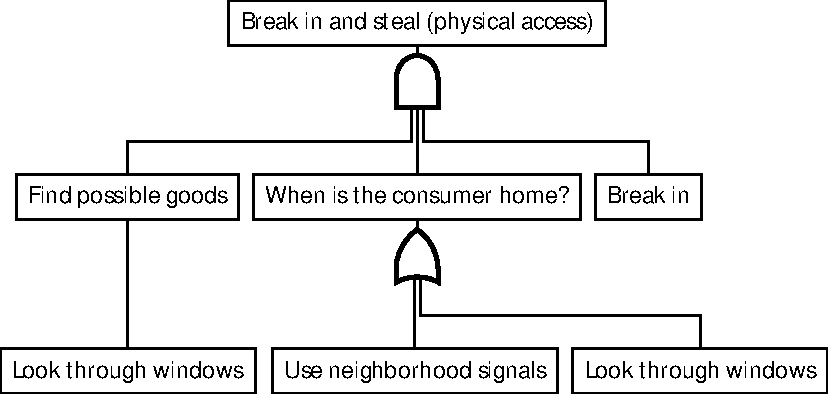
\includegraphics[width=10cm]{graphics/burglarPhysical}
\end{frame}

\begin{frame}\frametitle{Burglar Attack Trees}
\centering
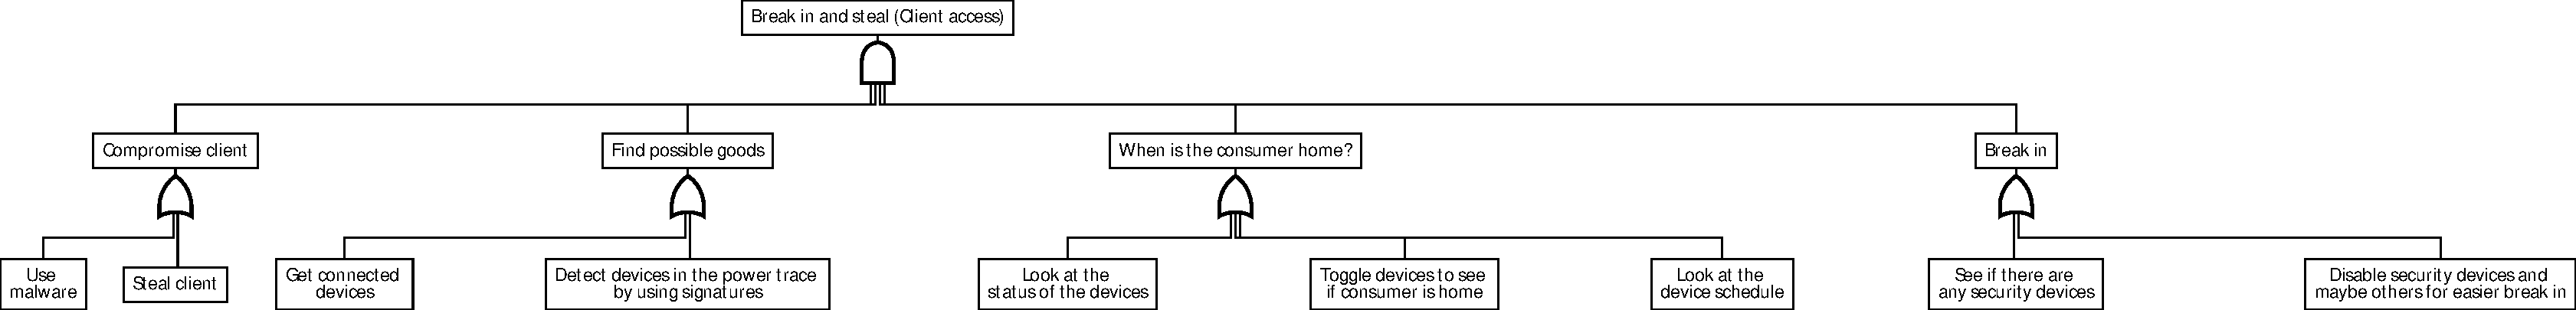
\includegraphics[width=11cm]{graphics/burglarClient}\\\vspace{0.5cm}
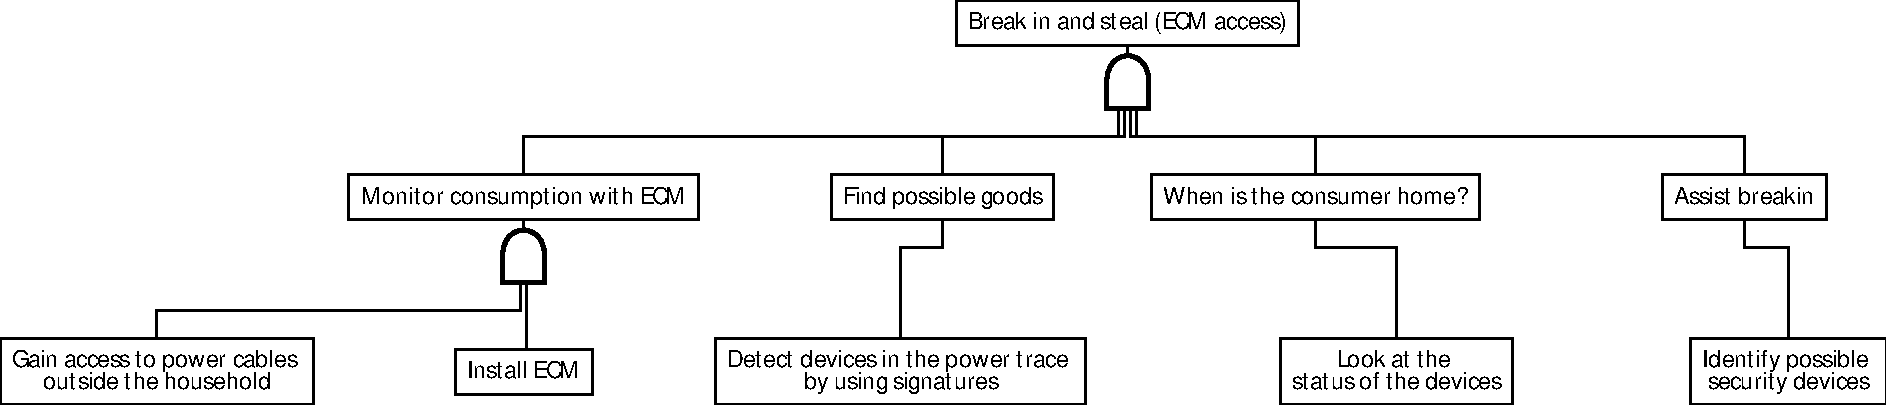
\includegraphics[width=11cm]{graphics/burglarECM}\\\vspace{0.5cm}
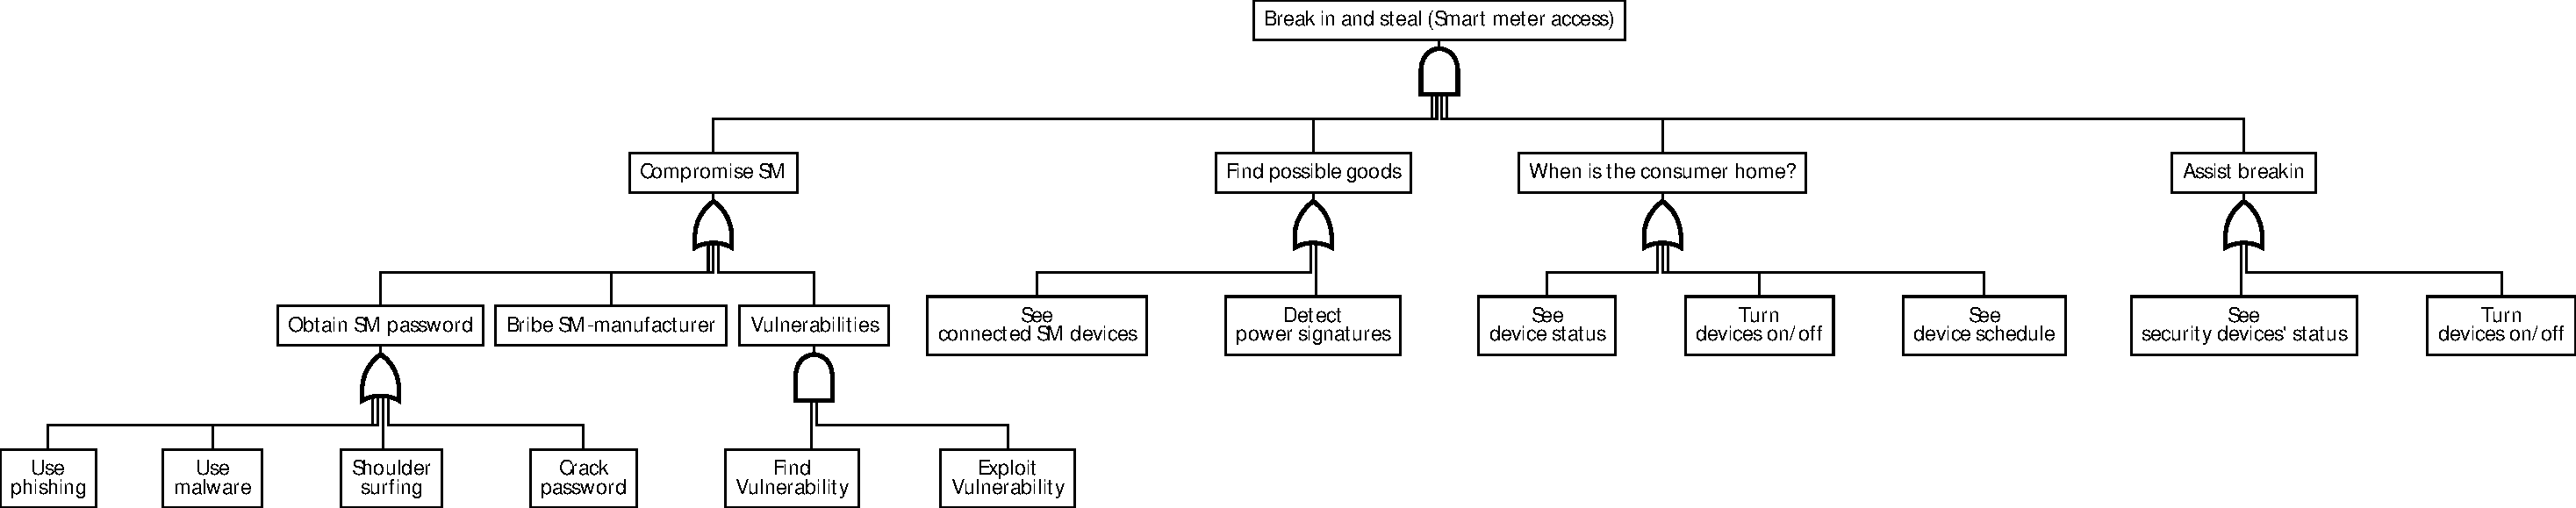
\includegraphics[width=11cm]{graphics/burglarSM}
\end{frame}

%Subtræer der giver adgang til noget forskelligt (SM, ECM, physical)

% Attack trees will describe the cause-effect relation between parts of an attack:
% I must do a before I do B.
% This describes the goal of the attack as well as any prerequisites for performing that specific attack.
% Problematic to represent the correlation between a cause and effect when intertwined

%Genbrug af subtræer, referencer (?)

% To solve the above (relation between cause and effect) subtrees could have been used.
% Subtrees could represent different groups of nodes, such as ways to gain access to the system or exploitations.
% The larger trees could then have been represented using combinations of these trees.
% This might have simplified the visual appearance of the large trees.

\begin{frame}\frametitle{Subtrees}
  \begin{block}{Causes and effects}
    \begin{itemize}
      \item Many trees include similar cause-effect relations
      \item Having multiple causes and effect complicates the structure
      \begin{itemize}
        \item If $A \rightarrow B$ and $C \rightarrow D$ it would be simpler to say $(A \vee C) \rightarrow (B \vee D)$
      \end{itemize}
      \item Trees are split on each cause-effect relation
    \end{itemize}
  \end{block}
  \begin{block}{References}
    \begin{itemize}
      \item Each cause and effect represented using a tree
      \item Relations identified by trees that link cause and effect
    \end{itemize}
  \end{block}
\end{frame}

%Størrelse -- bliver meget hurtigt store
%delebørn -- multiple parents

% Besides representing the order between a nodes elements (A before B), it might also be nice to show how one element is related to multiple elements.
% In the current representation you are required to look for these relations, instead of having them appear visually.
% Most of the trees were also generated using multiple parents - which did not provide much of an overview.

\begin{frame}\frametitle{Non-Trees}
  \begin{block}{Common dependency}
    \begin{itemize}
      \item Two nodes might require the same preceding step
      \begin{itemize}
        \item One cause can have two effects
      \end{itemize}
      \item Cannot be represented as a tree (one parent per child)
    \end{itemize}
  \end{block}
  \begin{block}{Graph representation}
    \begin{itemize}
      \item Joining multiple causes and effects into a single graph
      \item Difficult to follow the relations
      \item Does not clearly depict the threats when focusing on a single attack method
    \end{itemize}
  \end{block}
\end{frame}

\begin{frame}\frametitle{Scoring Trees}
  \begin{block}{Scoring parameters}
    \begin{itemize}
      \item Each element in a tree can be associated with a set of values
      \item Scores are weighed relatively given their \emph{``importance''}
      \item Scores can be associated with an attack or defense
      \begin{itemize}
        \item Cost (price in dollars) of hiring someone to carry out the task
        \item Time to carry out the attack
        \item Availability of countermeasures
      \end{itemize}
    \end{itemize}
  \end{block}
  \begin{block}{In this project}
    \begin{itemize}
      \item Not employed due to time-constraints
      \item Focus of project was to map the possible attacks
      \item Any future work on the attack trees could include scoring
    \end{itemize}
  \end{block}
\end{frame}
